\newpage
\subsection{Charakteristiken und Klassifikation von Gleichungssystemen 1. Ordnung}
\label{sec:3.2}
Ausgangspunkt: 
\begin{align}
\label{eq:6}
\bm{A}(\bm{x}(z,t))\frac{\partial \bm{x}(z,t)}{\partial z}+\bm{B}(\bm{x}(z,t))\frac{\partial \bm{x}(z,t)}{\partial t} = \bm{c}(\bm{x}(z,t),z,t)
\end{align}
\begin{align*}
\label{eq:6'}
\textrm{kurz: } \bm{A}\frac{\partial \bm{x}(z,t)}{\partial z}+\bm{B}\frac{\partial \bm{x}(z,t)}{\partial t}=\bm{c} \tag{6'}
\end{align*}
Annahme:
\begin{align*}
\det(\mu \bm{A}+ \nu \bm{B}) \neq 0 
\end{align*}
$\mu, \nu \in \R \rightarrow$ Regularität von \eqref{eq:6}.
Charakteristiken: 
Eine Kurve $\Gamma:s \mapsto (\alpha(s),\beta(s))=(z,t)$ ist eine charakteristische Projektion zu \eqref{eq:6}, wenn es nicht möglich ist aus
\begin{align} 
\label{eq:7}
\bm{x}(\alpha(s),\beta(s))=:\bm{h}(s)
\end{align}
die Ableitungen $\frac{\partial \bm{x}(z,t)}{\partial z}, \frac{\partial \bm{x}(z,t)}{\partial t}$ auf $\Gamma$ zu berechnen.
Differenzieren von \eqref{eq:7}:
\begin{align*}
\frac{\partial \bm{x}(\alpha(s),\beta(s))}{\partial z}\alpha'(s)+\frac{\partial \bm{x}(\alpha(s),\beta(s))}{\partial t}\beta'(s)=\bm{h}'(s)
\end{align*}
ergibt mit \eqref{eq:6'}
\begin{subequations}
\begin{align}
\bm{A}\frac{\partial \bm{x}}{\partial z}+\bm{B}\frac{\partial \bm{x}}{\partial t} =\bm{c}
\end{align}
\begin{align}
\alpha'\frac{\partial \bm{x}}{\partial z}+\beta'\frac{\partial \bm{x}}{\partial t} =\bm{h}'
\end{align}
\end{subequations}
Beobachtung: $\alpha', \beta'$ können nicht verschwinden.

Fall 1: $\alpha' \neq 0$
$(8a)\alpha-(8b)\bm{A}:(\alpha'\bm{B}-\beta'\bm{A})\frac{\partial \bm{x}}{\partial t}=\alpha'\bm{c}-\bm{A}\bm{h}'$

Fall 2: $\beta' \neq 0$
$(8a)\beta-(8b)\bm{B}:(\beta'\bm{A}-\alpha'\bm{B})\frac{\partial \bm{x}}{\partial z}=\beta'\bm{c}-\bm{B}\bm{h}'$

Damit $\frac{\partial \bm{x}}{\partial z}$ bzw. $\frac{\partial \bm{x}}{\partial t}$ nicht bestimmt werden können, muss gelten:
\begin{align}
\label{eq:9}
\det(\beta'\bm{A}-\alpha'\bm{B}) \overset{!}{=} 0
\end{align}
Für Charakterisierung wird folgender Spezialfall betrachtet:
Untersuchung der Kurve $s \mapsto (0,s)$. Diese Kurve soll keine Charakteristik sein.

\begin{figure}[ht]
	\centering
	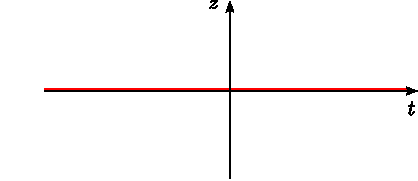
\includegraphics{img/keinecharakteristik}
	\label{fig:keinecharakteristik}
\end{figure}

Dann folgt für Charakteristik $\alpha(s) \neq 0$
$\underbrace{\Rightarrow}_{\eqref{eq:9}} $
Multiplikation von \eqref{eq:6} mit $\bm{A}^{-1}$
\begin{align*}
\pd{\bm{x}}{z}=-\underbrace{\bm{A}^{-1}\bm{B}}_{\bm{B}^*} \pd{\bm{x}}{t}+\underbrace{\bm{A}^{-1}\bm{c}}_{\bm{c}^*}
\end{align*}
aus \eqref{eq:9} folgt: 
\begin{align*}
\det(\beta'\bm{I}_n-\alpha'\bm{B}^*)=0
\end{align*}
da $a'\neq0$
\begin{align*}
\det\Big(\underbrace{\frac{\alpha'}{\beta'}}_{\lambda}\bm{I}_n-\bm{B}^*\Big)=0 \textrm{ mit } &\beta(s) = t(s) \quad \beta'=\frac{dt}{ds} \\ &\alpha(s) = z(s) \quad \alpha'=\frac{dz}{ds}
\end{align*}
$\lambda = \frac{dt}{dz}$ sind somit die Eigenwerte von $\bm{B}^*=\bm{A}^{-1}\bm{B}$.
Klassifikation:
\begin{itemize}
\item alle Eigenwerte sind komplex $\rightarrow$ elliptisches System (z.B. örtlich 2-dim stationäre Probleme, d.h. $t$ ist 2. Ortskoordinate)
\item alle Eigenwerte reel, zu jedem Eigenwert existiert ein Eigenvektor, $\bm{B}^*$ ist diagonalisierbar $\rightarrow$ hyperbolisches System
\item $\bm{B}^*$  besitzt nur einen reellen Eigenvektor $\rightarrow$ parabolisches System
\end{itemize}

parabolisch/hyperbolisch: dynamische Phänomene

Mischtypen möglich, physikalisch sinnvoll: hyperb.-parab.

\subsection{Klassifikation und Charakteristiken von Gleichungen 2. Ordnung}
Ausgangspunkt: Skalare pDgl. 2. Ordnung (jetz: Gl. 10)
\begin{align}
\label{eq:10}
a \frac{\partial^2 x}{\partial^2 z} + 2b \frac{\partial^2x}{\partial z\partial t} + c \frac{\partial^2 x}{\partial t^2} = d
\end{align}
($a,b,c,d$ hängen von $z,t,x,\frac{\partial x}{\partial z},\frac{\partial x}{\partial t}$ ab)

Vorgabe von $x,\frac{\partial x}{\partial z},\frac{\partial x}{\partial t}$ auf 
\begin{align*}
\Gamma:\R \rightarrow \R \times \R \textrm{ mit } s \mapsto (\alpha(s),\beta(s))=(z,t)
\end{align*}
mit 
\begin{subequations}
\begin{align}
\alpha(s),\beta(s)) = h(s) \label{eq:11a}\\
\frac{\partial x}{\partial z}(\alpha(s),\beta(s))=\phi(s) \label{eq:11b}\\
\frac{\partial x}{\partial t}(\alpha(s),\beta(s))=\psi(s) \label{eq:11c}
\end{align}
\end{subequations}
Frage: Wann können  $\frac{\partial^2 x(z,t)}{\partial z^2},\frac{\partial^2 x(z,t)}{\partial z \partial t}=\frac{\partial^2 x(z,t)}{\partial z \partial z},\frac{\partial^2 x(z,t)}{\partial t^2}$ auf $\Gamma$ aus $h,\phi, \psi$ berechnet werden?
Es gilt:
\begin{align*}
\eqref{eq:11a} \quad h'(s) &= \pd{\bm{x}}{z} \alpha' + \pd{\bm{x}}{t}\beta' = \varphi(s)\alpha'(s) + \psi(s)\beta'(s) \\
\eqref{eq:11b} \quad \varphi'(s) &= \pd[2]{\bm{x}}{z} \alpha' + \pd[2]{\bm{x}}{z\partial t}\beta' \\
\eqref{eq:11c} \quad \psi'(s) &= \pd[2]{\bm{x}}{z \partial t} \alpha' + \pd[2]{\bm{x}}{^2 t}\beta' \\
\end{align*}
aus \eqref{eq:11b}, \eqref{eq:11c} und \eqref{eq:10} folgt:
\begin{align}
\label{eq:12}
\underbrace{\begin{pmatrix}
a & 2b & c \\
\alpha' & \beta' & 0 \\
0 & \alpha'& \beta'
\end{pmatrix}}_{\bm{M}}\begin{pmatrix}
\pd[2]{\bm{x}}{z^2} \\ \pd[2]{\bm{x}}{z\partial t} \\ \pd[2]{\bm{x}}{t^2}
\end{pmatrix} =
\begin{pmatrix}
d \\ \varphi' \\ \psi'
\end{pmatrix}
\end{align}
charakteristisch $\Rightarrow \det(\bm{M})=0$
\begin{align}
\Rightarrow a \beta'^2 - 2b \alpha' \beta' + c \alpha'^2 = 0
\end{align}
Spezialfall (wie in \ref{sec:3.2}) Betrachtung von Charakteristiken mit $\alpha'(s) \neq 0$ und zusätzlich $z = \alpha(s)=s$
\begin{align*}
\Rightarrow &a \beta' - 2b \alpha' \beta' + c \alpha'^2 = 0 | \cdot \frac{1}{\alpha'}(=1) \\
&a \frac{\beta'^2}{\alpha'^2} - 2b \frac{\beta'}{\alpha'} + c = 0 \\
&a\lambda^2-2 b \lambda + c = 0 \\
&\lambda_{1/2}=\frac{b}{a} \pm \frac{\sqrt{b^2-ac}}{a}  
\end{align*}
\begin{align*}
&b^2-ac >0 \quad &\textrm{reelle Lsg., hyperbolisch} \\
&b^2-ac <0 \quad &\textrm{konj. kompl. Lsg., elliptisch} \\
&b^2=ac \quad &\textrm{parabolisch}
\end{align*}